\documentclass[review]{siamart190516}

% -----------------------------------------------------------------------------
% 1. Preamble and packages
\usepackage{amsfonts}
\usepackage{amsmath}
\usepackage{graphicx}
\usepackage{subfig}
\usepackage{epstopdf}
\usepackage{hyperref}
\ifpdf%
  \DeclareGraphicsExtensions{.eps,.pdf,.png,.jpg}
\else
  \DeclareGraphicsExtensions{.eps}
\fi
\usepackage{amsopn}
\DeclareMathOperator{\diag}{diag}
\usepackage{booktabs}

% Paper title
\newcommand{\TheTitle}{%
  Local Fourier Analysis of Balancing Domain Decomposition for High-Order Finite Element Operators
}

% Short title for running heads (if needed)
\newcommand{\TheShortTitle}{%
  LFA of BDDC for High-Order FEM
}

% Acknowledge funding or other resources
\newcommand{\TheFunding}{This work is supported by the Exascale Computing Project (17-SC-20-SC), a collaborative effort of two U.S. Department of Energy organizations (Office of Science and the National Nuclear Security Administration) responsible for the planning and preparation of a capable exascale ecosystem, including software, applications, hardware, advanced system engineering and early testbed platforms, in support of the nation’s exascale computing imperative.
}

% Authors: full names plus addresses.
\author{
  Jeremy L Thompson\thanks{Department of Applied Mathematics, University of Colorado, Boulder, CO
    (\email{jeremy@jeremylt.org}).}
  \and Jed Brown\thanks{Department of Computer Science, University of Colorado, Boulder, CO
    (\email{jed@jedbrown.org}).}
  \and Yunhui He\thanks{Department of Applied Mathematics, University of Waterloo, Waterloo, ON, Canada
    (\email{yunhui.he@uwaterloo.ca}).}
}
\newcommand{\TheShortAuthors}{
  J. L. Thompson, J. Brown, and Y. He
}

% Title and funding information on page
\title{{\TheTitle}\thanks{\TheFunding}}
\headers{\TheShortTitle}{\TheShortAuthors}

% Optional PDF information
\ifpdf
\hypersetup{
  pdftitle={\TheTitle},
  pdfauthor={\TheShortAuthors}
}
\fi
% -----------------------------------------------------------------------------

\begin{document}

\maketitle

\vspace{1cm}

% -----------------------------------------------------------------------------
\begin{abstract}
TODO
\end{abstract}
% -----------------------------------------------------------------------------

% -----------------------------------------------------------------------------
\begin{keywords}
  % Keywords that describe the paper
  local Fourier analysis, BDDC, high-order, finite elements
\end{keywords}
% -----------------------------------------------------------------------------

% -----------------------------------------------------------------------------
\section{Introduction}\label{sec:intro}
% -----------------------------------------------------------------------------

ToDo

This paper is organized as follows.
In \cref{sec:notation} we outline the notation for LFA used in this paper.
In \cref{sec:lfa} we develop the notation for LFA of second-order PDEs with arbitrary order bases, dimension, and number of components used in LFAToolkit.jl, and we use this notation to develop LFA of BDDC.
\Cref{sec:results} contains numerical results investigating the performance of BDDC on high and low-order elements for the two dimensional scalar Laplacian and three dimensional linear elasticity.
Finally, \cref{sec:conclusion} contains concluding remarks.

% -----------------------------------------------------------------------------
\subsection{Reproducibility}\label{sec:reproducibility}
% -----------------------------------------------------------------------------

The numerical results for LFA in this paper were generated using the Julia package LFAToolkit.jl \cite{thompson2021toolkit}.
This package is under active development and may be found on GitHub at \href{https://github.com/jeremylt/LFAToolkit.jl}{jeremylt/LFAToolkit.jl}.
This repository contains Julia scripts and interactive Jupyter notebooks that can replicate the tables and plots in this paper.

% -----------------------------------------------------------------------------
\section{Definitions and Notation}\label{sec:notation}
% -----------------------------------------------------------------------------

Consider a scalar Toeplitz operator $L_h$ on an infinite one dimensional uniform nodal grid $G_h$,
\begin{equation}
\begin{split}
L_h \mathrel{\hat{=}} \left[ s_\kappa \right]_h \left( \kappa \in V \right);\\
L_h w_h \left( x \right) = \sum_{\kappa \in V} s_\kappa w_h \left( x + \kappa h \right),
\end{split}
\end{equation}
where $V \subset \mathbb{Z}$ is a finite index set, $s_\kappa \in \mathbb{R}$ are constant coefficients, and $w_h \left( x \right)$ is a $l^2$ function on $G_h$. In the terminology of stencils, $s_{\kappa}$ are stencil weights that are nonzero on the neighborhood $\kappa \in V$.

Since $L_h$ is Toeplitz, it can be diagonalized by the standard Fourier modes $\varphi \left( \theta, x \right) = e^{\imath \theta x / h}$, which alias according to $\varphi(\theta+ 2\pi/h, x) = \varphi(\theta, x)$ on all grid points $x \in h \mathbb Z$.

\begin{definition}[Symbol of $L_h$]\label{def:symbol}
If for all grid functions $\varphi \left( \theta, x \right)$ we have
\begin{equation}
L_h \varphi \left( \theta, x \right) = \tilde{L}_h \left( \theta \right) \varphi \left( \theta, x \right),
\end{equation}
then we define $\tilde{L}_h \left( \theta \right) = \sum_{\kappa \in V} s_\kappa e^{\imath \theta \kappa}$ as the symbol of $L_h$, where $\imath^2 = -1$.
\end{definition}

This definition can be extended to a $q \times q$ linear system of operators by
\begin{equation}
\mathbf{L}_h =
\begin{bmatrix}
    L_h^{1, 1} && \cdots && L_h^{1, q}        \\
    \vdots               && \vdots && \vdots  \\
    L_h^{q, 1} && \cdots && L_h^{q, q}        \\
\end{bmatrix},
\end{equation}
where $L_h^{i, j}$, $i, j \in \lbrace 1, 2, \dots, q \rbrace$ are given by scalar Toeplitz operators describing how component $j$ appears in the equation for component $i$.
The components here may represent different fields and/or nodes of a finite element basis.
The symbol of $\mathbf{L}_h$, denoted $\tilde{\mathbf{L}}_h$, is a $q \times q$ matrix-valued function of $\theta$ given by $\left( \tilde{\mathbf{L}}_h \right)_{i, j} = \tilde{L}_h^{i, j} \left( \theta \right)$.
For a system of equations representing an error propagation operator in a relaxation scheme, the spectral radius of the symbol matrix determines how rapidly the scheme decreases error at a target frequency.

These definitions are readily extended to $d$ dimensions by taking the neighborhood $V \subset \mathbb Z^d$ and letting $\theta \in [-\pi,\pi)^d$.
For standard coarsening from fine $h=1$ to coarse $h=2$, low frequencies are given by $\theta \in T^{\text{low}} = \left[ - \pi / 2, \pi / 2 \right)^d$ and high frequencies are given by $\theta \in \left[-\pi, \pi \right)^d \setminus T^{\text{low}}$ or equivalently by periodicity, $\theta \in T^{\text{high}} = \left[ - \pi / 2, 3 \pi / 2 \right)^d \setminus T^{\text{low}}$.

% -----------------------------------------------------------------------------
\section{Local Fourier Analysis for Balancing Domain Decomposition by Constraints}\label{sec:lfa}
% -----------------------------------------------------------------------------

We now describe the LFA formulation used in LFAToolkit.jl, first in one dimension and then in multiple dimensions, followed by LFA of BDDC with high-order finite elements.

% -----------------------------------------------------------------------------
\subsection{High-Order Finite Elements}\label{sec:highorder}
% -----------------------------------------------------------------------------

We will use the representation of the weak form of linear second-order PDEs described in \cite{brown2010efficient}, which is given by
\begin{equation}
\langle v, f \left( u \right) \rangle = \int_{\Omega}
\begin{bmatrix}
  v^T & \nabla v^T    \\
\end{bmatrix}
\begin{bmatrix}
  f_{0, 0} & f_{0, 1} \\
  f_{1, 0} & f_{1, 1} \\
\end{bmatrix}
\begin{bmatrix}
  u                   \\
  \nabla u            \\
\end{bmatrix}
= \int_{\Omega} f v,\quad \forall v \in \mathcal V
\end{equation}
for some suitable $\mathcal V \subseteq H_0^1 \left( \Omega \right)$.
In this equation, $f_{i, j}$ may come from a linear PDE or the linearization of a non-linear problem.
Boundary terms have been omitted, as they are not present on the infinite uniform grid $G_h$.

Selecting a finite element basis, we can discretize this weak form and produce
\begin{equation}\label{pdediscrete}
\mathbf{A} \mathbf{u} = \mathbf{b}.
\end{equation}

Using the algebraic representation of PDE operators given in \cite{brown2010efficient}, the PDE operator $\mathbf{A}$ is of the form
\begin{equation}\label{efficienthighorder}
\mathbf{A} = \mathbf{G}^T \mathbf{A}_e \mathbf{G},\quad \text{with} \,\,\mathbf{A}_e = \mathbf{B}^T \mathbf{D} \mathbf{B},
\end{equation}
where $\mathbf{G}$ represents the element assembly operator, $\mathbf{B}$ is a basis operator which computes the values and derivatives of the basis functions at the quadrature points, and $\mathbf{D}$ is a block diagonal operator which provides the pointwise application of the bilinear form on the quadrature points, to include quadrature weights and the change in coordinates between the physical and reference space.

Consider the specific case of a block Toeplitz operator representing an arbitrary second order scalar PDE in one dimension with Lagrange basis of polynomial degree $p$ given in the form of \cref{pdediscrete} and \cref{efficienthighorder}.
The basis $\mathbf{B}$ is defined on the mesh grid with points given by $x_i$, for $i \in \left\lbrace 1, 2, \dots, p + 1 \right\rbrace$ on one element.
The nodes on the left and right boundaries of the element map to the same Fourier mode when localized to nodes unique to a single finite element, so we can compute the symbol matrix of size $p \times p$ as
\begin{equation}\label{symbolscalar1d}
\tilde{\mathbf{A}} = \mathbf{Q}^T \left( \mathbf{A}_e \odot \left[ e^{\imath \left( x_j - x_i \right) \theta / h} \right] \right) \mathbf{Q},
\end{equation}
where $\odot$ represents pointwise multiplication of the elements, $h$ is the length of the element, and $i, j \in \lbrace 1, 2, \dots, p + 1 \rbrace$.
In the pointwise product $\mathbf{A}_e \odot \left[ e^{\imath \left( x_j - x_i \right) \theta / h} \right]$, the $\left( i, j \right)$ entry is given by $\left( \mathbf{A}_e \right)_{i, j} e^{\imath \left( x_j - x_i \right) \theta / h}$.
$\mathbf{Q}$ is a $\left( p + 1 \right) \times p$ matrix that localizes Fourier modes to each finite element, given by
\begin{equation}
\mathbf{Q} =
\begin{bmatrix}
    \mathbf{I}   \\
    \mathbf{e}_0 \\
\end{bmatrix} =
\begin{bmatrix}
    1      && 0      && \cdots && 0      \\
    0      && 1      && \cdots && 0      \\
    \vdots && \vdots && \vdots && \vdots \\
    0      && 0      && \cdots && 1      \\
    1      && 0      && \cdots && 0      \\
\end{bmatrix}.
\end{equation}
We refer to $\mathbf{Q}$ as the Fourier mode localization operator.

The computation of this symbol matrix extends to more complex PDE with multiple components and in higher dimensions.
Multiple components are supported by extending the $p \times p$ system of Toeplitz operators in \cref{symbolscalar1d} to a $\left( n \cdot p \right) \times \left( n \cdot p \right)$ system of operators, where $n$ is the number of components in the PDE.
The localization operator for a multi-component PDE is given by $\mathbf{Q}_n = \mathbf{I}_n \otimes \mathbf{Q}$, where $I_n$ is the identity matrix with size $n \times n$.
In general, we omit the subscript indicating the number of components for the localization operator.

The infinite uniform grid $G_h$ is extended into higher dimensions by taking the direct sum of the one dimensional grid.
Tensor products are used to extend the one dimensional bases into higher dimensions.
The basis evaluation operators in two dimensions are given by
\begin{equation}
\begin{split}
\mathbf{B}_{\text{interp2d}} = \mathbf{B}_{\text{interp1d}} \otimes \mathbf{B}_{\text{interp1d}}, \\
\mathbf{B}_{\text{grad2d}} =
\begin{bmatrix}
    \mathbf{B}_{\text{grad1d}} \otimes \mathbf{B}_{\text{interp1d}} \\
    \mathbf{B}_{\text{interp1d}} \otimes \mathbf{B}_{\text{grad1d}} \\
\end{bmatrix},
\end{split}
\end{equation}
where $\mathbf{B}_{interp*d}$ and $\mathbf{B}_{grad*d}$ are the basis interpolation and gradient operators, respectively.

In a similar fashion, the localization operator for Fourier modes in two dimensions is given by
\begin{equation}
\mathbf{Q}_{\text{2d}} = \mathbf{Q} \otimes \mathbf{Q}.
\end{equation}
As with tensor product bases, an analogous computation can be done in higher dimensions.
Again, we generally omit the subscript indicating the dimension of the Fourier mode localization operator.

\begin{definition}\label{def:high_order_symbol}
The symbol matrix of a finite element operator for an arbitrary second order PDE with any basis order, dimension, and number of components is given by
\begin{equation}\label{symbolhighorder}
\tilde{\mathbf{A}} = \mathbf{Q}^T \left( \mathbf{A}_e \odot \left[ e^{\imath \left( \mathbf{x}_j - \mathbf{x}_i \right) \cdot \boldsymbol{\theta} / \mathbf{h}} \right] \right) \mathbf{Q},
\end{equation}
where $\odot$ represents pointwise multiplication of the elements, $\mathbf{h}$ is the length of the element in each dimension, $\boldsymbol{\theta}$ is the target frequency in each dimension, $i, j \in \lbrace 1, 2, \dots, n \cdot \left( p + 1 \right)^d \rbrace$, $n$ is the number of components, $p$ is the polynomial degree of the discretization, and $d$ is the dimension of the finite element basis.
$\mathbf{A}_e$ is the finite element operator for the element and $\mathbf{Q}$ is the localization of Fourier modes on an element.
\end{definition}

Note that this LFA notation is applicable to any second-order PDE with a weak form that can be represented by \cref{efficienthighorder}.
This representation is used in LFAToolkit.jl, where the users provide the finite element basis $\mathbf{B}$, the node to mode mapping $\mathbf{Q}$, and the pointwise representation of the weak form $\mathbf{D}$, and the software can provide the LFA of the PDE with various preconditioners.
The nodes may be defined by points $\mathbf x_i$ or more generally, as dual basis functions that may be applied to the Fourier modes; however, we restrict ourselves to nodal bases in this paper.

If the pointwise representation of the weak form $\mathbf{D}$ has a tensor product structure, then the element operator $\mathbf{A}_e$ and therefore the symbol $\tilde{\mathbf{A}}$ will have a tensor product structure, as shown in \cite{he2020two}.
We omit this optimization in this analysis and LFAToolkit.jl in favor of supporting second-order PDEs that do not have a tensor product decomposition.

% -----------------------------------------------------------------------------
\subsection{Balancing Domain Decomposition by Constraints}\label{sec:lfabddc}
% -----------------------------------------------------------------------------

With this representation of the symbol of high-order PDE operators, we can derive the symbol of BDDC preconditioned operators.

ToDo

% -----------------------------------------------------------------------------
\subsubsection{Subassembled Symbol}\label{sec:lfasubassembled}
% -----------------------------------------------------------------------------

ToDo

% -----------------------------------------------------------------------------
\subsubsection{Injection Symbols}\label{sec:lfainjection}
% -----------------------------------------------------------------------------

ToDo

% -----------------------------------------------------------------------------
\subsection{Extension to Macro-Elements}\label{sec:previouswork}
% -----------------------------------------------------------------------------

ToDo

% -----------------------------------------------------------------------------
\section{Numerical Results}\label{sec:results}
% -----------------------------------------------------------------------------

In this section, we present validation with previous numerical results for this analysis for the scalar Laplacian in two dimensions with $H^1$ Lagrange bases on Gauss-Lobatto points with Gauss-Legendre quadrature.

% -----------------------------------------------------------------------------
\subsection{Scalar Laplacian - Low-Order Validation}\label{sec:lowordervalidate}
% -----------------------------------------------------------------------------

Previous work by Brown, He, and MacLachlan \cite{brown2019local} provided LFA of lumped and Dirichlet BDDC on subdomains consisting of multiple low-order finite elements.
This previous work provided very sharp LFA convergence estimates when compared to numerical experiments with PETSc \cite{petsc-user-ref} on a periodic mesh.

\begin{table}[ht!]
\begin{center}
\begin{tabular}{l ccc ccc}
  \toprule
  $m$  &  \multicolumn{3}{c}{Lumped BDDC}  &  \multicolumn{3}{c}{Dirichlet BDDC}  \\
  %\cmidrule(lr){2-3} \cmidrule(lr){4-5} \cmidrule(lr){6-7}
                      &  $\lambda_{\min}$  &  $\lambda_{\max}$  &  $\kappa$ & $\lambda_{\min}$  &  $\lambda_{\max}$ & $\kappa$  \\
  \toprule
  $m = 4$   &  1.000  &   4.444  &   4.444  &  1.000  &  2.351  &  2.351  \\
  $m = 8$   &  1.000  &  12.269  &  12.269  &  1.000  &  3.196  &  3.196  \\
  $m = 16$  &  1.000  &  31.179  &  31.179  &  1.000  &  4.188  &  4.188  \\
  $m = 32$  &  1.000  &  75.761  &  75.761  &  1.000  &  5.335  &  5.335  \\
  \bottomrule
\end{tabular}
\end{center}
\caption{Condition Numbers and Maximal Eigenvalues for Low-Order Macro-Elements}
\label{table:macro_element_bddc}
\end{table}

\cref{table:macro_element_bddc} shows the maximal eigenvalues and condition numbers for the symbol of the BDDC preconditioned operator $\tilde{\mathbf{M}}^{-1}_i \left( \boldsymbol{\theta} \right) \tilde{{\color{burgundy}\mathbf{A}}} \left( \boldsymbol{\theta} \right)$ for the two dimensional Poisson problem on linear macro-element subdomains with varying numbers of elements in one dimension.
The maximal eigenvalues were computed across $64$ uniformly spaced frequencies.
These values exactly agree with the previous work by Brown, He, and MacLachlan \cite{brown2019local}.

It is important to note the significantly improved condition number and resulting improved convergence for the Dirichlet BDDC.
Lumped BDDC has approximately half of the setup costs when compared to Dirichlet BDDC when using assembled exact inverses.
Brown, He, and MachLachlan investigated the use of multiplicative combinations of the lumped BDDC operator with a diagonal scaling operator to improve convergence while still retaining the benefit of cheaper setup for lumped BDDC.
This technique helped mitigate the growth of the condition number for the lumped BDDC as the subdomain size grew, but the resulting condition number was still larger than the condition number for Dirichlet BDDC.

% -----------------------------------------------------------------------------
\subsection{Scalar Laplacian - High-Order Validation}\label{sec:highordervalidate}
% -----------------------------------------------------------------------------

Single high-order elements can represent an equivalent number of degrees of freedom.
This approach has been investigated for solid mechanics problems, such as in \cite{pavarino2010bddc}; although, this work incorporated additional primal degrees of freedom from average values across subdomain edges and faces.

\begin{table}[ht!]
\begin{center}
\begin{tabular}{l ccc ccc}
  \toprule
  $p$  &  \multicolumn{3}{c}{Lumped BDDC}  &  \multicolumn{3}{c}{Dirichlet BDDC}  \\
                      &  $\lambda_{\text{min}}$  &  $\lambda_{\text{max}}$  &  $\kappa$ & $\lambda_{\text{min}}$  &  $\lambda_{\text{max}}$ & $\kappa$  \\
  \toprule
  $p = 2$   &  1.000  &    2.800  &    2.800  &  1.000  &  2.042  &  2.042  \\
  $p = 4$   &  1.000  &   12.948  &   12.948  &  1.000  &  3.242  &  3.242  \\
  $p = 8$   &  1.000  &   59.563  &   59.563  &  1.000  &  5.197  &  5.197  \\
  $p = 16$  &  1.000  &  289.678  &  289.678  &  1.000  &  7.761  &  7.761  \\
  \bottomrule
\end{tabular}
\end{center}
\caption{Condition Numbers and Maximal Eigenvalues for Single High-Order Element Subdomains}
\label{table:high_order_element_bddc}
\end{table}

\cref{table:high_order_element_bddc} shows the maximal eigenvalues and condition numbers for the symbol of the BDDC preconditioned operator $\tilde{\mathbf{M}}^{-1}_i \left( \boldsymbol{\theta} \right) \tilde{{\color{burgundy}\mathbf{A}}} \left( \boldsymbol{\theta} \right)$ for the two dimensional Poisson problem on single high-order element subdomains with varying polynomial orders.

The improved condition number, and therefore convergence, of the Dirichlet BDDC compared to the lumped BDDC is more significant for high-order elements.
With single high-order element subdomains, the Fast Diagonalization Method approximate inverse subdomain solver can be used for both the subdomain subassembled inverse and subdomain interior inverse, which eliminates the advantage in reduced setup costs for lumped BDDC.

\begin{figure}[!ht]
  \centering
  \subfloat[Lumped BDDC]{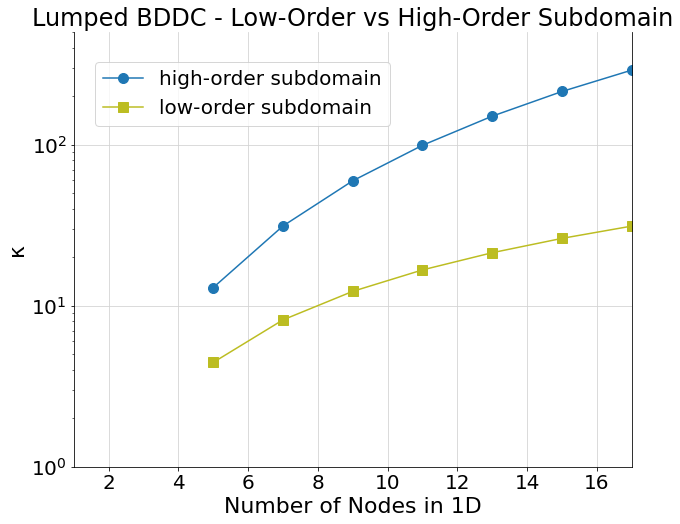
\includegraphics[width=0.48\textwidth]{img/lowVsHighLumped}\label{fig:lumped_bddc_comparison}}
  \hfill
  \subfloat[Dirichlet BDDC]{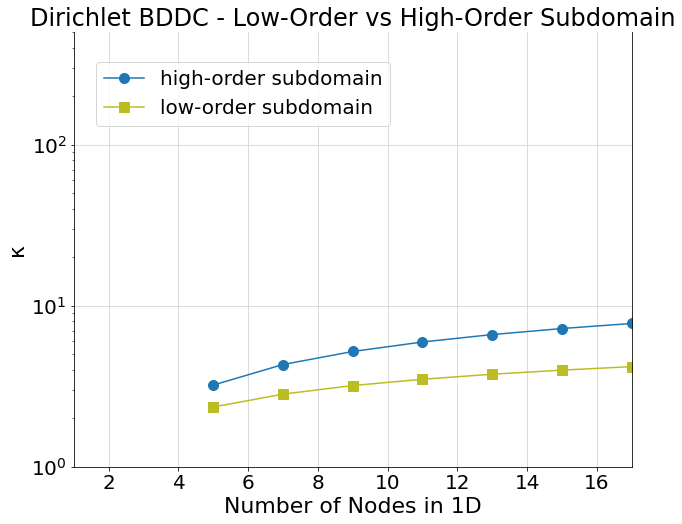
\includegraphics[width=0.48\textwidth]{img/lowVsHighDirichlet}\label{fig:dirichlet_bddc_comparison}}
  \caption{Low-Order and High-Order Subdomain Condition Number Comparison}
\end{figure}

In \cref{fig:lumped_bddc_comparison} we compare the growth of the condition number for the lumped BDDC preconditioned operator for a subdomain consisting of several linear elements and a subdomain consisting of a single high-order element for the two dimensional Poisson problem.
The condition number grows much more rapidly for a high-order subdomain with an equivalent number of degrees of freedom.

In \cref{fig:dirichlet_bddc_comparison} we compare the growth of the condition number for the Dirichlet BDDC preconditioned operator for a subdomain consisting of several linear elements and a subdomain consisting of a single high-order element for the two dimensional Poisson problem.
In contrast with Figure \ref{fig:lumped_bddc_comparison}, we see that the condition number of the preconditioned operator on the high-order subdomain grows only slightly faster than the condition number of the low-order subdomain.

\begin{figure}[!ht]
  \centering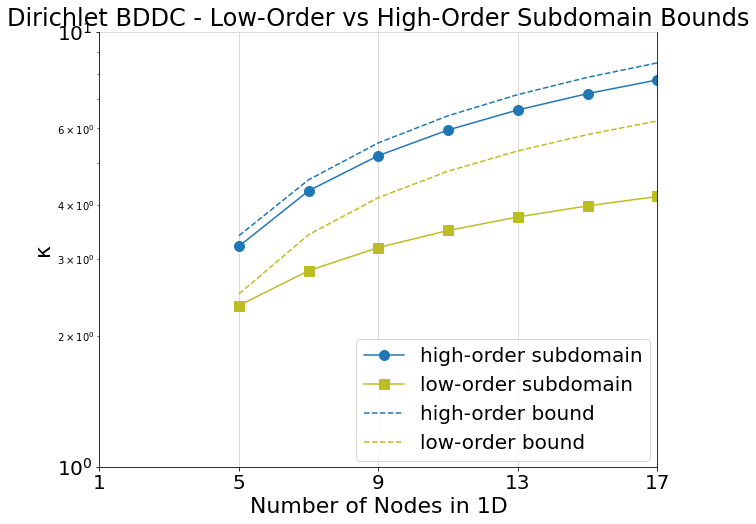
\includegraphics[width=0.48\textwidth]{img/lowVsHighDirichletBounds}
  \caption{Low-Order and High-Order Subdomain Condition Number Bounds}
  \label{fig:dirichlet_bddc_bounds}
\end{figure}

The condition numbers of the Dirichlet BDDC preconditoner operator is bounded by
\begin{equation}
\kappa \leq \mathcal{C} \left( 1 + \log \left( p^2 \frac{H}{h} \right) \right)^2
\end{equation}
where $\mathcal{C} > 0$ is independent of the polynomial order $p$, the element size $h$, and the subdomain size $H$ \cite{klawonn2008spectral}.
In Figure \ref{fig:dirichlet_bddc_bounds}, we can see that our LFA-predicted condition numbers closely agree with this bound.

Klawonn, Pavarino, and Rheinbach investigated the performance of BDDC and FETI-DP preconditioners for the two dimensional Poisson problem with discontinuous coefficients \cite{klawonn2008spectral} and provided some experimentally derived maximal eigenvalues and condition numbers for the two dimensional Poisson problem.

\begin{table}[ht!]
\begin{center}
\begin{tabular}{l ccc ccc}
  \toprule
  $p$  &  \multicolumn{3}{c}{LFA}  &  \multicolumn{3}{c}{Experimental Results}  \\
                      &  $\lambda_{\text{min}}$  &  $\lambda_{\text{max}}$  &  $\kappa$ & $\lambda_{\text{min}}$  &  $\lambda_{\text{max}}$ & $\kappa$  \\
  \toprule
  $p = 2$   &  1.000  &   2.042  &   2.042  &  1.001  &   1.66  &   1.66  \\
  $p = 3$   &  1.000  &   2.614  &   2.614  &  1.000  &   2.38  &   2.38  \\
  $p = 4$   &  1.000  &   3.241  &   3.241  &  1.001  &   3.03  &   3.03  \\
  $p = 8$   &  1.000  &   5.195  &   5.194  &  1.001  &   5.01  &   5.00  \\
  $p = 16$  &  1.000  &   7.756  &   7.756  &  1.001  &   7.62  &   7.61  \\
  $p = 32$  &  1.000  &  10.961  &  10.961  &  1.002  &  10.86  &  10.84  \\
  \bottomrule
\end{tabular}
\end{center}
\caption{Condition Numbers and Maximal Eigenvalues for Dirichlet BDDC with Single Element High-Order Subdomains}
\label{table:high_order_bddc_experiments_1}
\end{table}

\begin{table}[ht!]
\begin{center}
\begin{tabular}{l ccc ccc}
  \toprule
  $p$  &  \multicolumn{3}{c}{LFA}  &  \multicolumn{3}{c}{Experimental Results}  \\
                      &  $\lambda_{\text{min}}$  &  $\lambda_{\text{max}}$  &  $\kappa$ & $\lambda_{\text{min}}$  &  $\lambda_{\text{max}}$ & $\kappa$  \\
  \toprule
  $p = 2$   &  1.000  &   2.700  &   2.700  &  1.001  &   2.33  &   2.33  \\
  $p = 3$   &  1.000  &   3.568  &   3.568  &  1.001  &   3.21  &   3.21  \\
  $p = 4$   &  1.000  &   4.305  &   4.305  &  1.002  &   4.00  &   3.99  \\
  $p = 8$   &  1.000  &   6.511  &   6.511  &  1.003  &   6.26  &   6.24  \\
  $p = 16$  &  1.000  &   9.354  &   9.354  &  1.002  &   9.16  &   9.14  \\
  $p = 32$  &  1.000  &  12.856  &  12.856  &  1.002  &  12.69  &  12.66  \\
  \bottomrule
\end{tabular}
\end{center}
\caption{Condition Numbers and Maximal Eigenvalues for Dirichlet BDDC 4 Element High-Order Subdomains}
\label{table:high_order_bddc_experiments_2}
\end{table}

In \cref{table:high_order_bddc_experiments_1} we see the LFA-predicted maximal eigenvalues and condition numbers for the scalar Poisson problem in two dimensions with constant coefficients compared to numerical results on a domain with 576 subdomains consisting of a single high-order finite element.
The LFA-predicted condition numbers generally agree with the experimental results, typically providing a mildly pessimistic prediction when compared to the experimental results.

In \cref{table:high_order_bddc_experiments_1} we see the LFA-predicted maximal eigenvalues and condition numbers for the scalar Poisson problem in two dimensions with constant coefficients compared to numerical results on a domain with 576 subdomains consisting of four high-order finite elements.

% -----------------------------------------------------------------------------
\subsection{Linear Elasticity - 3D Convergence Factors}\label{sec:solidsresults}
% -----------------------------------------------------------------------------

ToDo

% -----------------------------------------------------------------------------
\section{Conclusions}\label{sec:conclusion}
% -----------------------------------------------------------------------------

In this paper we developed LFA of BDDC with arbitrary second-order PDEs using high-order finite element discretizations by using an operator representation for efficient application of matrix-free implementations.
We used LFAToolkit.jl to investigate BDDC on high-order elements and validate against previous work.

The LFA of p-multigrid framework presented here can be extended to the LFA of BDDC on low-order finite elements and reproduces previous work in this area.

% -----------------------------------------------------------------------------
\bibliographystyle{siamplain}
\bibliography{../references}
% -----------------------------------------------------------------------------

\end{document}

% -----------------------------------------------------------------------------
